%
% To use this as a template for turning in your solutions, change the flag
% \inclsolns from 0 to 1. Make sure you include macros.tex in the directory
% containing this file. Edit the "author" and "collaborators" fields as
% appropriate. Write your solutions where indicated.
%

\documentclass[11pt]{article}

\usepackage{fullpage}
\usepackage{graphicx}
\usepackage{enumerate}
\usepackage{comment}
\usepackage{amsmath,amssymb,amsthm}
\usepackage{hyperref}
\usepackage[capitalise]{cleveref}
\usepackage{todonotes}

\usepackage[
backend=biber,
style=alphabetic,
sorting=ynt
]{biblatex}
\addbibresource{refs.bib}

\newtheorem{theorem}{Theorem}
\newtheorem{conjecture}[theorem]{Conjecture}
\newtheorem{lemma}[theorem]{Lemma}
\newtheorem{proposition}[theorem]{Proposition}
\newtheorem{corollary}[theorem]{Corollary}
\newtheorem{claim}[theorem]{Claim}
\newtheorem{fact}[theorem]{Fact}
\newtheorem{openprob}[theorem]{Open Problem}
\newtheorem{remk}[theorem]{Remark}
\newtheorem{apdxlemma}{Lemma}
\theoremstyle{definition}
\newtheorem{definition}[theorem]{Definition}
\newtheorem{example}[theorem]{Example}
\newtheorem{problem}{Problem}

\newenvironment{remark}{\begin{remk}

\begin{normalfont}}{\end{normalfont}
\end{remk}}
\newtheorem{sublemma}[theorem]{Sublemma}


%%%%%%%%%%%%%%%%%%%%%%% text macros
\newcommand{\etal}{{\it et~al.\ }}
\newcommand{\ie} {{\it i.e.,\ }}
\newcommand{\eg} {{\it e.g.,\ }}
\newcommand{\cf}{{\it cf.,\ }}

%%%%%%%%%%%%%%%%%%%%%%% general useful macros
\newcommand{\eqdef}{\mathbin{\stackrel{\rm def}{=}}}
\newcommand{\R}{{\mathbb R}}
\newcommand{\N}{{\mathbb{N}}}
\newcommand{\Z}{{\mathbb Z}}
\newcommand{\F}{{\mathbb F}}
\newcommand{\poly}{{\mathrm{poly}}}
\newcommand{\polylog}{{\mathrm{polylog}}}
\newcommand{\loglog}{{\mathop{\mathrm{loglog}}}}
\newcommand{\zo}{\{0,1\}}
\newcommand{\suchthat}{{\;\; : \;\;}}
\newcommand{\pr}[1]{\Pr\left[#1\right]}
\newcommand{\deffont}{\em}
\newcommand{\getsr}{\mathbin{\stackrel{\mbox{\tiny R}}{\gets}}}
\newcommand{\E}{\mathbb{E}}
\newcommand{\Var}{\mathop{\mathrm Var}\displaylimits}
\newcommand{\eps}{\varepsilon}
\newcommand{\one}{\mathbf{1}}

%%%%%%%%%%%%%%%%%%%%%%%%%% linear algebra
\newcommand{\rank}{\operatorname{rank}}
\newcommand{\spn}{\operatorname{span}}

%%%%%%%%%%%%%%%%%%% macros particular to this course

\newcommand{\mathprob}[1]{\mathsf{#1}}
\newcommand{\SAT}{\mathprob{SAT}}
\newcommand{\yes}{{\sc yes}}
\newcommand{\no}{{\sc no}}

\newcommand{\class}[1]{\mathbf{#1}}
\newcommand{\TIME}{\class{DTIME}}
\newcommand{\NTIME}{\class{NTIME}}
\renewcommand{\P}{\class{P}}
\newcommand{\NP}{\class{NP}}
\newcommand{\coNP}{\class{coNP}}
\newcommand{\BPP}{\class{BPP}}
\newcommand{\BQP}{\class{BQP}}
\newcommand{\RP}{\class{RP}}
\newcommand{\coRP}{\class{coRP}}
\newcommand{\ZPP}{\class{ZPP}}
\newcommand{\MA}{\class{MA}}
\newcommand{\AM}{\class{AM}}
\newcommand{\Sigmacc}[1]{\class{\Sigma^p_{#1}}}
\newcommand{\Picc}[1]{\class{\Pi^p_{#1}}}
\newcommand{\SZK}{\class{SZK}}
\newcommand{\PP}{\class{PP}}
\newcommand{\sharpP}{\class{\#P}}
\newcommand{\IP}{\class{IP}}
\newcommand{\Ecc}{\class{E}}
\newcommand{\EXP}{\class{EXP}}
\newcommand{\NEXP}{\class{NEXP}}

\newcommand{\SPACE}{\class{SPACE}}
\newcommand{\NSPACE}{\class{NSPACE}}
\renewcommand{\L}{\class{L}}
\newcommand{\NL}{\class{NL}}
\newcommand{\coNL}{\class{coNL}}
\newcommand{\BPL}{\class{BPL}}
\newcommand{\RL}{\class{RL}}
\newcommand{\PSPACE}{\class{PSPACE}}

\newcommand{\Ppoly}{\class{P_{/poly}}}
\newcommand{\AC}{\class{AC}}
\newcommand{\NC}{\class{NC}}
\newcommand{\ACC}{\class{ACC}}

\newcommand{\PCP}{\class{PCP}}

\newcommand{\negl}{{\mathrm{neg}}}
\newcommand{\sgn}{\operatorname{sgn}}

\newcommand{\Enc}{\operatorname{Enc}}
\newcommand{\Dec}{\operatorname{Dec}}

%%%%%%Gates%%%%%%%%
\newcommand{\THR}{\mathrm{THR}}
\newcommand{\MAJ}{\mathrm{MAJ}}
\newcommand{\AND}{\mathrm{AND}}
\newcommand{\OR}{\mathrm{OR}}
\newcommand{\XOR}{\mathrm{XOR}}

%%%%%%%Functions%%%%%
\newcommand{\EQ}{\mathrm{EQ}}
\newcommand{\GT}{\mathrm{GT}}



%If you want to add more macros, do it like this
\newcommand{\dolphin}{\mathsf{DOLPHIN!!}}
\newcommand{\PPAD}{\mathsf{PPAD}}
\newcommand{\FP}{\mathsf{FP}}
\newcommand{\FNP}{\mathsf{FNP}}
\newcommand{\PPADc}{\mathsf{PPAD}\text{-complete}}
\newcommand{\NASH}{\mathsf{NASH}}
\newcommand{\eNASH}{\mathsf{\text{$\epsilon$-}NASH}}
\newcommand{\rNASH}{\mathsf{\text{$r$-}NASH}}
\newcommand{\eol}{\mathsf{EOL}}
\newcommand{\seol}{\mathsf{SEOL}}



\author{Bassel El Mabsout$^1$, Nicolas AlHaddad$^1$}

% on the computational complexity of nash equilibria
\title{On the computational complexity of computing an approximate Nash equilibrium}
\date{November 17, 2020}

\begin{document}
	\maketitle
	\footnotetext[1]{Authors contributed equally}
\section{Introduction}

% What are the main contributions of the paper you are reviewing? This introduction should emphasize conceptual contributions and why they are important, avoiding technical definitions and details:\\
Game theory is a theoretical framework for modeling the strategic interactions among rational decision-makers, allowing us to study the science of logical decision making in humans, animals, and computers.
The Nash equilibrium is a central concept in game theory used for predicting the behavior of such systems in terms of searching for an optimal strategy. It therefore touches a huge array of problems in, Social Science, economics, systems science and Computer Science. This paper discusses the computational complexity of finding Nash equilibria in games as it has direct implications on the plausibility of it being a good model for the behavior of real systems. Intuitively, if the fastest computers cannot compute it within many universe lifetimes, then how can we hope that a group of real agents would do so.


John Nash showed \cite{Nash48} that every game has at least 1 mixed Nash equilibrium but proved it non-constructively leaving open the problem of whether there exists an efficient algorithm to compute it. A Nash equilibrium is
a stable state of a game, where no participant can gain by changing their strategy if the strategies of the others remain the same. It is called mixed when those strategies are represented by probability distributions.

In the beginning John von Neumann showed \cite{NeumannZurTD} that the problem of finding the Nash equilibrium in a 2 player game where the sum of the payoffs is 0 for any strategy (think rock-paper-scissors where the loser pays the winner 1\$, no matter what everyone chooses their total sum of money remains unchanged, meaning no new money is added or removed from the system) can be found in polynomial time on a deterministic Turing machine through the famous mini-max algorithm (computable polynomially in the size of the description of the game). In more complex scenarios such as with more players or non-zero-sum games, however, it remained an open problem whether one can always find such Nash equilibria efficiently. 

This motivated the creation of the class called $\PPAD$ \ref{PPAD} (polynomial parity argument for directed graphs). A canonical language that is $\PPADc$ is $\eol$ (Definition \ref{eol}). Interestingly, finding a Nash equilibrium ($\NASH$) was not proven to be $\PPADc$ immediately. The first paper shows \cite{daskalakis2009complexity} that even $\eNASH$ (Definition \ref{eNash}) (which is $\NASH$ but approximated with $\epsilon = 1/2^{poly(n)}$ precision where $n$ is the input size describing the game) with more than 2 players is $\PPADc$. Shortly after, another paper by Chen, Deng and Teng \cite{chen2007settling} extended this result for 2 players. Meaning that finding the equilibria of games in general is most likely more difficult than the 2-player zero-sum game case (and indeed even for $>2$-player zero-sum games this problem is $\PPADc$ \cite{cai2011minmax}).



\subsection{Outline}
In Section 2 we give all the definitions and background required to prove the main result of the original paper\cite{daskalakis2009complexity}. In Section 3 we go through the proofs of why $\eNASH$ is $\PPADc$. In Section 4 we provide a discussion about future work. Finally, in Section 5 we criticize the original paper \cite{daskalakis2009complexity}.
% end of line problem they say it's obvious we do it.
\section{Preliminaries}

$\PPAD$ is a class of search problems that is conjectured to be hard. A search problem is defined as a set of functions: $F:\{\zo^* \to \zo^*\}$. $\FP$ is defined as the subset of $F$ such that every $f \in \FP$ is computable with a deterministic polytime Turing machine. Equivalently, $\FNP$ is defined as the subset of $F$ such that every $f \in \FNP$ is computable with a non-deterministic polytime Turing machine. Consequently $\FP \subseteq \FNP$ analogous to the corresponding decision problems $\P \subseteq \NP$ ($\FP = \FNP \iff \P = \NP$). It turns out that $\FP \subseteq \PPAD \subseteq \FNP$, and it is likely that $\FP \subsetneq \PPAD$ because if $\PPAD \subseteq \FP$ then $\NP = \coNP$ \cite{daskalakis2009complexity}.

\begin{definition}
    \label{PPAD}
    $\PPAD$: is the class of all search problems that are poly-time reducible to $\eol$ (Definition \ref{eol}). This makes $\eol$ trivially $\PPADc$. $\PPAD$ was introduced by Papadimitriou in 1994 \cite{PAPADIMITRIOU1994498} so that he can study the computational complexity of NASH equilibrium.
    $\PPAD$ stands for the polynomial parity argument on directed graphs and it is based on the fact that every directed graph with an unbalanced vertex (it's unbalanced when the number of incoming edges $\not =$ outgoing edges) must also contain at least one other unbalanced vertex as well. The corresponding search problem is to find such a vertex ($\eol$). Notice that since such a vertex always exist, this makes $\PPAD$ a class of total functions (search problems).
    Alternatively, A binary relation P(x,y) is in $\PPAD$ if and only if there is a deterministic polynomial time algorithm that can determine whether P(x,y) holds given both x and y, and for every x, there exists a y such that P(x,y) holds based on a parity argument on directed graphs.\\
\end{definition}

\begin{definition}
\label{GAME}
GAME: A game in normal form has has at least 2 players. Each player in the game must have a finite a set of strategies associated with that player denoted by $S_p$. The set of all strategies in the game is the Cartesian product of all personal strategies and is denoted by $S$. To refer to all strategies except for the strategies of player p they denote that by $S_{-p}$. To refer to a subset T of player strategies in S, they denote that by $S_T$. To denote the payoff or utility of a certain strategy of a player $p$ (the value of an outcome when player p choose a certain strategy $s$ from $S$, notice that the utility is calculated by also looking at other players strategies, because $S$ is the Cartesian product of all players strategies). They refer to this by ${u^p_s}$ and in normal form they assume that the payoff should always be $\ge 0$.
\end{definition}

\begin{definition}
    \label{NASH}
    Nash equilibrium: Each player chooses a probability distribution over their $S_p$ (see definition \ref{GAME}), called a mixed strategy, so that no player can deviate from their mixed strategy and improve on their expected payoff, i.e. "no unilateral player has incentive to deviate". The authors do give a detailed algebraic definition of the problem but we omit it for the sake of brevity (and clarity). Also notice, that the solution to $\NASH$ (the probabilities chosen by the players) might be irrational, if that's the case then computers have to approximate that value (they have finite precision) as they can't compute the exact NASH equilibrium.
\end{definition}
\begin{definition}
    \label{eNash}
    $\eNASH$: If Nash equilibrium means “no incentive to deviate,” then approximate Nash equilibrium stands for “low incentive to deviate”.
    Specifically, if $\epsilon$ is a small positive quantity, we can define an $\eNASH$ equilibrium as a profile of mixed strategies where any player can improve their expected payoff by at most $\epsilon$ by switching to another strategy.
    
\end{definition}

\begin{definition}
\label{rNash}
$\rNASH$ is the problem of finding $\NASH$ with $\epsilon$ accuracy in a game that has $r$ players.
It's a search problem that is guaranteed to have a solution \cite{Nash48}.
\end{definition}

\begin{definition}
    \label{eol}
    $\eol$ (End-of-Line): G is a (possibly exponentially large) directed graph specified by a poly-time computable function $f$ (for example defined implicitly by a poly-sized circuit) with no isolated vertices:\\
    Input: A description of a directed  graph G and a specified unbalanced vertex of G.\\
    Output: Some other unbalanced vertex.\\
    As mentioned in the description of $\PPAD$ (Definition \ref{PPAD}), any graph containing an unbalanced vertex must also contain another.
    Intuitively, every source must have a sink (otherwise it wouldn't be a source) and $\eol$ is the problem of finding a sink.\\
    Note: One may think that this class is easy to solve, one would assume that a simple graph traversal algorithm will be enough to find the other vertex. However, we can't afford to do the graph traversal if the graph itself is exponentially large and we are given a description of that graph. Remember G can be specified by a poly sized circuit but the graph itself can be exponential!
\end{definition}

\begin{definition}
    \label{seol}
    $\seol$ (Simplified-End-of-Line):\\
    This is the same definition of $\eol$ but restricted so that every vertex in $G$ has at most 1 outgoing vertex and at most 1 incoming vertex (this definition is often used as the definition of $\eol$ \cite{chen2007settling}) and $f$ is represented by a circuit  C with $n$ inputs such that when given the index of a vertex, it outputs the index of the vertex that it points to (when the index of a vertex is given to $C$ and it maps to its self, this means it doesn't point at anything). Because the structure of $G$ means that vertices with only one neighbour come in pairs, this keeps the problem $\PPADc$. In particular, given a source $s$, we can find a sink $s'$ at the other end of the path starting at s. (Note that this may take exponential time if we just evaluate $f$ repeatedly)
\end{definition} 

\begin{theorem}
    \label{Brouwer}
    Brouwer's fixed-point theorem \cite{Brouwer} states that for any continuous function $f$ mapping a compact convex set to itself there is a point $x_0$ such that $f(x_0) = x_0$, the corresponding problem of finding such a fixed point is denoted as $\mathsf{BROUWER}$ \cite{PAPADIMITRIOU1994498} and as they proved, it is $\PPADc$ (Definition \ref{Brouwerc}). As an example lets take the disk in $\mathbb{R}^2$ where $x^2 + y^2 \leq 1$. Let our continuous transformation $f$ be a rotation of the disk so that for every point $(x,y)$ satisfying the constraint $x^2 + y^2 \leq 1$ will map to some point satisfying the same constraint (A.K.A. it maps the disk to itself). According to this theorem, there must exist at least a point that didn't change through the transformation. Note that since we're doing a rotation here and the disk stays `in the same spot', then this forces our rotation to be about the point $(0,0)$ (our fixed point).\\
    In the paper they solve their version of Brouwer which is a discrete and simplified version of the search problem associated with Brouwer’s fixed point theorem and they define it formally as: \\
    Brouwer Input: An  efficient  algorithm  $\Pi_F$ for  the  evaluation of a function $F: [0,1]^m \longrightarrow [0,1]^m$; a constant K such  that F satisfies the Lipschitz condition (Definition \ref{lip});  and  the  desired accuracy $\epsilon$.\\
    Output: A point x such that $d(F(x),x) \le \epsilon$
    This definition is motivated by the fact that representing irrational numbers is computationally intractable. Since $F$ maps $[0,1]^m$ to its self, there is no guarantee that fixed points will be rational therefore a specific accuracy $\epsilon$ is required. The Lipschitz condition guarantees that any point close to the fixed point will remain in a region determined by $\epsilon$, $K$ and $m$. Meaning that the approximation guarantees completeness (when a fixed point exists in an $\epsilon$ sized region then any point within that region will map to some other point in this same region). 
    % Basically, they turned finding a Brouwer fixed point of a function into a combinatorial problem by introducing approximation.
\end{theorem}

\begin{definition}
\label{lip}
     Lipschitz condition over an $m$-hypercube: $F$ satisfies this condition if $\exists K,\forall x_1, x_2 \in [0,1]^m, d(F(x_1),F(x_2)) \leq K*d(x_1,x_2)$, where $d$ is defined as the Euclidean distance. And $x_1,x_2$ are points in the $[0,1]$ subset of euclidean space of $m$ dimensions ($m$-hypercube). For example, the linear function F(x) = x that is defined over the domain $[0,1]$ $(m=1)$, we can see that $d(F(x_1), F(x_2)) = d(x_1,x_2) \le k * d(x_1,x_2)$ for $k \geq 1$. Hence, F satisfies the condition.\\
\end{definition}

\begin{lemma}
    \label{Sperner}
    Sperner's lemma \cite{SpernerNeuerBF}: Combinatorial analog of the Brouwer fixed point theorem. The lemma states that every Sperner coloring of a triangulation of an n-dimensional simplex contains a cell colored with a complete set of colors. The grid in Figure \ref{fig:triangulated} is colored according to a Sperner coloring. Notice, there exist triangles with vertices colored with all set of three colors (these are the shaded triangles).
    
\end{lemma}

\begin{figure}[h!]
    \centering
    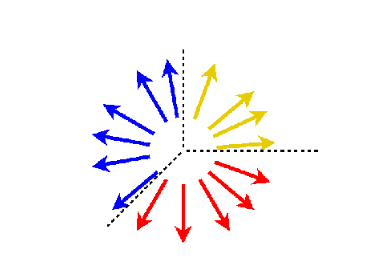
\includegraphics[width=0.3\textwidth]{project/color_assignment.png}
    \caption{The colors assigned to the different directions of $F(x)-x$.  There is a transition from red to yellow  at 0 degrees,  from  yellow  to  blue at 90 degrees, and from blue to red at 225 degrees.}
    \label{fig:color_assignment}
\end{figure}

\begin{figure}[h!]
    \centering
    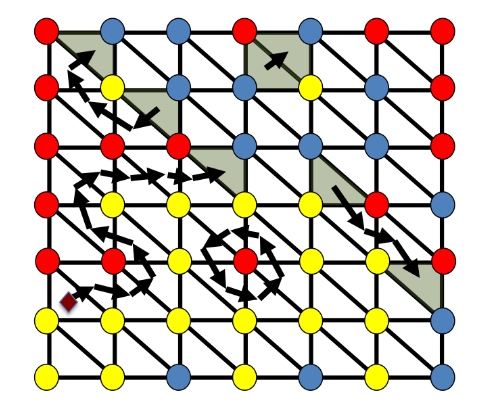
\includegraphics[width=0.5\textwidth]{project/triangulation_square.png}
    \caption{The subdivision of the square into smaller squares, and the coloring of the vertices of the subdivision according to the direction of $F(x) - x$.  The arrows correspond to the $\eol$ graph on the triangles of the subdivision; the source T is marked by a diamond}
    \label{fig:triangulated}
\end{figure}
\newpage
\section{Main Results}

The main result of the paper is showing that $\rNASH$ is $\PPADc$ for players $r \ge 3$. The paper we are summarizing is the 2009 paper where they updated their result, they also mention that it is possible for $r = 2$ as well. Warning: The proofs used here rely heavily on topology!

% \begin{enumerate}
% \item First, they show that $\mathsf{BROUWER}$ is $\PPADc$. By doing a polytime reduction from  $\mathsf{BROUWER}$ to $\eol$ and then from $\eol$ back to $\mathsf{BROUWER}$.
% \end{enumerate}
\begin{lemma}
    \label{Brouwerc}
     $\mathsf{BROUWER}$ is $\PPADc$
\end{lemma}
\begin{proof}
    To prove that $\mathsf{BROUWER}$ is $\PPADc$ they prove that $\mathsf{BROUWER} \in \PPAD$ and that $\mathsf{BROUWER}$ is $\PPAD$-hard.
    \begin{enumerate}
        \item $\mathsf{BROUWER} \in \PPAD$: This is done through reduction from $\mathsf{BROUWER}$ to $\eol$. Since $\eol \in \PPAD$ then $\mathsf{BROUWER}\in \PPAD$:\\
            

            
            They take an instance of $\mathsf{BROUWER}$ (Definition \ref{Brouwer}) $F$  and build an input to $\eol$ (Definition \ref{eol}), mainly a Graph and an unbalanced vertex to start the end of line search from. Focusing on the 2d case, they discretize the $[0,1]^2$ square (domain of F) by forming a grid made of smaller squares (of side length determined by K and $\epsilon$),  and  then  divide  each little square into two right triangles. Notice that we can find approximate fixed points by searching for points that remained within the same triangle after the transformation. Meaning the size of the triangle determines the accuracy of the approximation. Since they're working in a discrete setting, they use the discrete analog of Brouwer's theorem, otherwise known as Sperner's Lemma \ref{Sperner}. Then, a Sperner coloring of this grid is performed: ``We  color  each  vertex of  the  triangles  by  one  of  three colors  depending  on  the direction in  which F maps x. In two dimensions, this can be taken to be the angle between vector $F(x)-x$ and the horizontal.  Specifically, we color it red if the direction lies between 0 and -135 degrees, blue if it ranges between 90 and 225 degrees, and yellow otherwise,as shown in Figure \ref{fig:color_assignment}.  (If the direction is 0 degrees, we allow either yellow or red;  similarly for the other two borderline cases.)  Using the above coloring convention the vertices get colored in such a way that the Lipschitz (Definition \ref{lip}) property is satisfied. None of the vertices on the lower side of the square uses red, no vertex on the left side uses blue, and no vertex on the other two sides uses yellow. Figure \ref{fig:triangulated} shows a coloring of the vertices that could result from the function F". Since this is a Sperner coloring, by Sperner's lemma (Definition \ref{Sperner}), this guarantees that there exists a triangle where the vertices are all colored differently (these are shaded in Figure \ref{fig:triangulated}). This indicates that within this triangle there is a fixed point. They reduce the problem of finding this triangle to $\eol$. There is always a path through the edges starting from the one going from yellow to red on the leftmost vertical line of the grid from which we can reach a tricolored triangle in the following way: From a red-yellow edge $e$ we reach another one $e'$ that is not visited before on the triangles connected to $e$. Once such an $e'$ does not exist, the corresponding triangle will be tricolored. Now, we can do a poly-time transformation of this graph into an input accepted by $\eol$ such that the source would be the starting edge on the left and the destination would be the edge of the tricolored triangle containing the fixed point (this is a slightly simplified but equivalent version of the rules in the paper). The transformation converts edges into vertices, triangles into edges such that the algorithm solving $\eol$ in the new graph would solve $\mathsf{BROUWER}$ in the old one.
        
        \item $\mathsf{BROUWER}$ is $\PPAD$-hard: In the paper they reduce $\eol$ to $\mathsf{BROUWER}$. $\eol$ is $\PPADc$ which implies that $\mathsf{BROUWER}$ is $\PPAD$-hard.\\
            The authors prove this by a poly-time transformation from any graph $G$ and source $s$ taken as inputs of $\eol$ to a computable $K$-Lipschitz continuous function $F$ mapping the 3-cube: $[0,1]^3$ to it's self where every fixed point is a sink and the source $s$ is a specific point in the cube. This transformation however is quite complex, we therefore present a simpler proof by replacing $\eol$ with $\seol$ and similarly polynomially reducing the problem of finding a vertex in our simpler $G$ with no outgoing edges (the end of the line) to finding a fixed point for a computable $K$-Lipschitz continuous function $F$ mapping $[0,1]$ to its self as follows:
            
                The number of vertices in $G$ cannot be larger $2^n$ ($n$ being the number of inputs to the circuit $C$ describing $G$). There is therefore a bijection between every vertex $v$ in $G$ and a point $p$ in the set $P: \{0,1/2^n, 2/2^n, \dots 1-1/2^n\}$ lying in our [0,1] region. Then, we define our computable transformation $F$ on every such $p$ by mapping it to the point $p' = p + 1/2^n$ if $C(p) \not = p$ otherwise $p' = p$. Notice that since $C$ maps vertex indices to themselves if they don't have an outgoing edge then every sink is mapped to a fixed point of $F$ and every other point is not. Now $F$ still needs to be a $K$-Lipschitz continuous total function over its domain, and to preserve this property every point in between the points in $P$ is linearly interpolated: For every point $x$ in $[0,1]$ lets define $\underline{x} = \frac{\lfloor x2^n \rfloor}{2^n}$. Then $F(x) = F(\underline{x}) + 2^n(x - \underline{x})(F(\underline{x} + 1/2^n) - F(\underline{x}))$, $F(1) = 1-2/2^n$ (to handle the special case of points between $1-2^n$ and $1$). Notice that for any $x_1, x_2 \in [0,1]$, $d(F(x_1), F(x_2)) \leq d(x_1, x_2)$ meaning our Lipschitz constant is 1. Also due to our mapping, any time a point $x$ has the property: $|x - F(x)| < 1/2^n$ will be a point where $\underline{x}$ is a fixed point making it obvious that finding an $\epsilon < 1/2^n$ approximated fixed point means finding the vertex in the graph that corresponds to a sink. This therefore concludes our proof that $\seol$ is poly-time reducible to $\mathsf{BROUWER}$.
    \end{enumerate}
    

\end{proof}
\begin{lemma}
    $\eNASH \leq_p \mathsf{BROUWER}$    
\end{lemma}
\begin{proof}
    The full proof from $\NASH$ to $\mathsf{BROUWER}$ was given by NASH  himself in the 1950: \cite{Nash48}. The paper argues that given that there is a reduction from $\NASH$ to $\mathsf{BROUWER}$ then there must a be reduction from $\eNASH \leq_p \mathsf{BROUWER}$.
    The idea behind Nash’s proof is to construct a function f from the set all of all strategies to itself, that satisfies the conditions of Brouwer’s fixed point theorem such that the fixed point x is a Nash equilibrium.  Unless the players are happy with x (which means they have reached nash equilibrium). The players will keep changing x. This function will indicate the movement of the unsatisfied players.
\end{proof}


\begin{lemma}
    $\mathsf{BROUWER} \leq_p \rNASH$ where $r=3$    
\end{lemma}
\begin{proof}
The key thing that the paper did is show how to make $\NASH$ games compute simple arithmetic functions and then use that to compute $\mathsf{BROUWER}$ functions. To do this they represented each arithmetic operation by a game of maximum of four players and then compose those games so that a Nash equilibrium in the final game represents an approximate fixed point in the original $\mathsf{BROUWER}$ function. We can represent any $\mathsf{BROUWER}$ function by a composition of these simple operators: addition, multiplication and comparison.  Addition and multiplication is easy to simulate by a game (by inducing a player to pick an action with probability that is the sum or the product of 2 other player's probability of picking that action. On a high level, the system is giving incentive for the players to produce the right answer to the arithmetic operation at hand). However, comparison requires special handling, the details of which are in the paper. Since circuits are inherently composable, if we replace every operation by a game. Then the composition of those games (through using 2 players as inputs and a third player as an output) is going to give the same result as the circuit.\\
However, we now have a problem. The number of operations in the circuit will dictate how many players we have in the final composed game. Notice, that many of the players within the games that represent arithmetic operations are independent in the sense that they don't effect each other's strategies. In particular this structure forms what is known as a graphical game. Graphical games can always be simulated by a game of three players. Hence, $\mathsf{BROUWER}$ is as difficult as computing $\rNASH$ with three players.
\end{proof}

% \begin{theorem}
%     $\eNASH$ is $\PPADc$ for $k > 2$
% \end{theorem}
% n particular, the reductions by Bubelis [ V. Bubelis. “On Equilibria in Finite Games,”International Journal of Game Theory, 8(2):65–79, 1979] in the 1970s comprise a remarkable early precursor of our work; it is astonishing that these important results had not been pursued for three decades. Bubelis established that the Nash equilibrium problem for 3players captures the computational complexity of the same problem with any number of players. In Section 4 we show the same resultin an indirect way, via the Nash equilibrium problem for graphical games — a connection that is crucial for our PPAD-completeness reduction. Bubelis also demonstrated in [5] that any algebraic number can be the basis of a Nash equilibrium, something that follows easily from our results(Theorem 14)
% \begin{proof}
    
% \end{proof}

\section{Conclusion}
It seems that computing Nash equilibria may be difficult since $\eNASH$ is $\PPADc$. Actually, there has been many improvements over what we know about the complexity of finding Nash equilibria. For instance, In this paper \cite{chen2007settling} they improve both the number of players required to play the game to the minimum possible of 2, and the approximation $\epsilon$ from $1/2^{poly(n)}$ in this paper to $1/poly(n)$ in theirs. But still, in order to discount $\NASH$ as a model, one has to prove that weakening the approximation even further would still be outside of $\FP$. And even if it is, it could still be tractable by being computable using quasi-polynomials, as far as we know, this remains an open problem. Another avenue to explore is whether we can exploit the structure of realistic games further generating a subset of games where finding the Nash equilibrium is in $\FP$. This is not unlikely as the algorithms with worst-case exponential time complexity often end up being efficient when applied on real problems.

\section{Critiques}
\begin{itemize}
    \item Notational abuse: The authors override the conventional definition of $\P$ and $\NP$ where it seems they mean $\FP$ and $\FNP$ instead. ``We think of $\NP$ as the class of search problems", this contradicts with the definitions provided in class where $\P$ and $\NP$ define the class of decision problems that can be solved with a polynomial time deterministic and non-deterministic Turing machine respectively.
    \item Zero-sum games are easy: The paper implies that finding the equilibrium of all zero-sum games can be done in poly-time. ``if  a  game  is  zero-sum, like the rock-paper-scissors game, then it follows from the work of John von Neumann in the 1920s that Nash can be  formulated  in  terms  of  linear  programming  (a  subject identified by George Dantzig in the 1940s); linear programs can be solved efficiently". This is misleading as it has been shown that the problem of finding the Nash equilibria of 3-player zero-sum-games is $\PPADc$. This is true only when the zero-sum game involves 2 players.
    \item $\epsilon$ confusion: The paper defines $\NASH$ as the problem of finding an approximate Nash equilibrium in a game with $\epsilon = 1/2^{poly(n)}$ where n is the input length. However, they also define $\eNASH$ to mean the same problem but where $\epsilon = 1/poly(n)$. Both definitions have to deal with approximations, since in the case of mixed equilibrium, the values may be irrational and we cannot have infinite precision on a DTM. Calling one $\eNASH$ and the other $\NASH$ is misleading.
\end{itemize}

% I like to use bibtex to organize reference, but you can use whatever you like. https://dblp.org/ is a good source for bibtex entries for CS papers
% \bibliographystyle{alpha}
% \bibliography{term_paper_bib}
\medskip

\printbibliography

\end{document}


